
\documentclass[english]{article}
%\documentclass[aps,pra,twocolumn,english]{revtex4}
%\documentclass[english]{iopart}
\usepackage[T1]{fontenc}
\usepackage[latin9]{inputenc}
\usepackage{babel}
\usepackage{graphicx,amsmath,amssymb,color}
\usepackage[normalem]{ulem}
\usepackage{amsfonts}
\usepackage[toc,page]{appendix}
%\usepackage[ocgcolorlinks,colorlinks=true,linkcolor=blue,citecolor=red]{hyperref}
\usepackage{hyperref}
\usepackage{latexsym}
\usepackage{amsfonts}
\usepackage{algpseudocode}
\usepackage{amsthm}
\usepackage{mathrsfs}
\usepackage{natbib}
\usepackage{color,verbatim}
\usepackage{psfrag}
\bibliographystyle{unsrt}
%\bibliographystyle{acm}
%\bibliographystyle{unsrtnat}
%\usepackage[style=numeric]{biblatex}

\usepackage{subcaption} % allows for subfigures


\usepackage[svgnames]{xcolor}
\usepackage{tikz}

\usepackage{algorithm}


%\input{tikzit/tikz_preamble.tex}  % load separately defined tikz preamble


\newcommand{\bra}[1]{\langle#1 |}
\newcommand{\ket}[1]{|#1 \rangle}
\newcommand{\braket}[2]{\left \langle #1 \mid #2 \right \rangle}
\newcommand{\bigbraket}[2]{\left \langle #1 \middle\vert #2 \right \rangle}
\newcommand{\ketbra}[2]{\vert #1 \rangle \! \langle #2 \vert}
\newcommand{\overlap}[2]{\left \langle #1 | #2 \right\rangle}
\newcommand{\average}[1]{\langle #1 \rangle}
\newcommand{\sandwich}[3]{\left \langle #1 \mid #2 \mid #3 \right\rangle}
\newcommand{\innerprod}[2]{\left \langle #1 | #2 \right\rangle}

\begin{document}


\title{Optical parametric oscillators and coherent Ising machines}
\author{Nicholas Chancellor}


\maketitle


\today % added for drafting, remove in final version


{\small Disclaimer: lecture notes may contain ``typo'' type errors (factors of $2$, minus signs, etc...) if something like this looks wrong there is a good chance it is, please let me know}

These notes are based partially on ``Nonlinear Optics'' by Robert Boyd ISBN: 978-0-12-369470-6, available for purchase at\footnote{while this is a good book in general I don't necessarily think that everyone needs a copy of  it the way we all have a copy of G+K (get QCI to buy you one if you don't already have it), maybe only get it if you want to know how the experiments work}:\\ \href{https://www.elsevier.com/books/nonlinear-optics/boyd/978-0-12-369470-6}{https://www.elsevier.com/books/nonlinear-optics/boyd/978-0-12-369470-6} as well as Gerry and Knight, coherent Ising machine discussion based on papers especially Yamamoto et.~al.~npj Quantum Information volume 3, Article number: 49 (2017) \href{https://doi.org/10.1038/s41534-017-0048-9}{https://doi.org/10.1038/s41534-017-0048-9}.


\section{Motivation}
\begin{itemize}
\item Optical parametric oscillators (and amplifiers) are important components in many quantum optics systems, it is therefore worth devoting a whole set of notes to them
\item Some of the ideas around thresholds in these systems are transferable to many others such as lasers
\item Coherent Ising machines are a model of quantum\footnote{or classical in many of the real implementations, explained later in the notes} computation which uses photons to solve problems stated as Ising models, if we don't explain carefully, people will just assume that the EQC is a coherent Ising machine, to show the difference we need to know how a coherent Ising machine works.
\item The way in which the mode of operation of the large scale coherent Ising machines currently in existence is not meaningfully quantum is a useful study in what to avoid if you want to make a truly quantum computer\footnote{This goal shouldn't be assumed always, it could be interesting (and profitable) to build unconventional \emph{classical} computers if they can improve computation in a meaningful way}
\item There is significant similarity in the structure of a coherent Ising machine and the RPC, although the purposes are quite different
\end{itemize}

\section{Optical parametric amplification}
\begin{itemize}
\item Consider a non-linear crystal with the following non-linear Hamiltonian \footnote{$s$, $p$ and $i$ stand for ``pump'', ``signal'', and ``idler'' respectively, the reason for this terminology is mostly historical, but it is widely used (including G+K), so I will use it to, Boyd tends to use 1,2,3} 
\begin{equation}
\hat{H}=\chi^{(2)}\left(\hat{a}_p\hat{a}^\dagger_s\hat{a}^\dagger_i+\hat{a}^\dagger_p\hat{a}_s\hat{a}_i\right)
\end{equation}
\item $\chi^{(2)}$ is usually small in practice, but if a large number of photons are already present, say in mode $p$, than the overall contribution can be significant, since the effective strength the other two modes see will scale as $\sqrt{n_p}$ 
\item When acting on a number state $\hat{a}_p\hat{a}^\dagger_s\hat{a}^\dagger_i$ will give a matrix element proportional to $\sqrt{n_p(n_s+1)(n_i+1)}$, therefore more photons in mode $i$ mean that more photons will be created in mode $i$ (and $s$)
\item Lets consider the case where $n_p\gg n_s$ and $n_p \gg n_i$ since the square root function is concave, than for any $n>m\ge1$ $\sqrt{n-1}\sqrt{m+1}>\sqrt{n}\sqrt{m}$, therefore even if the photons in mode $s$ quickly leave the material, the action of $\hat{a}_p\hat{a}^\dagger_s\hat{a}^\dagger_i$ will lead to faster creation of photons in $i$ and $s$ (and therefore absorption of $p$), of course this effect is even more dramatic if both are retained
\item Effectively the crystal can amplify an optical signal in mode $i$ and create a matching signal in mode $s$, and as long as the $p$ is not too depleted this effect gets stronger the longer the light travels through the material
\item If we assume that the absorption of photons from $p$ can be ignored, and both $s$ and $i$ remain in the material, than the number of photons in $s$ and $i$ will grow exponentially as the photons travel
\item This effect can be made even stronger by adding a cavity which causes photons in mode $i$ (or even both $i$ and $s$) to pass through the medium multiple times, this device is known as an \textbf{optical parametric oscillator} 

\begin{centering}
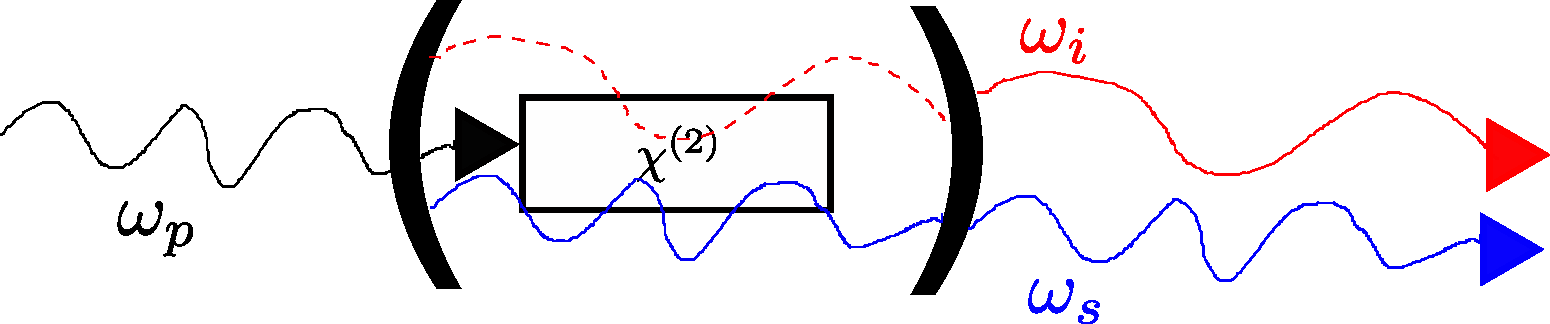
\includegraphics[width=10cm]{OPO_schematic}
\par
\end{centering}
\end{itemize}

\section{Optical parametric oscillator (OPO)}
\begin{itemize}
\item There are three types of optical parametric oscillators often considered
\begin{enumerate}
\item Singly resonant:  either mode $s$ or mode $i$, are significantly trapped by the cavity, but not both
\item Doubly resonant: both $s$ and $i$ are significantly trapped by the cavity, but they are both distinct modes
\item Degenerate: $s$ and $i$ are identical modes (i.e. the terms become $\left(\hat{a}_p\hat{a}^\dagger_s\hat{a}^\dagger_s+\hat{a}^\dagger_p\hat{a}_s\hat{a}_s\right)$) and significantly trapped by the cavity
\end{enumerate}
\item In all of these cases, there is an interesting tipping point: the point where photons in $s$ and $i$ are created faster than they are lost to the cavity, this is known as a \textbf{threshold}, below the threshold the OPO will act as an amplifier, above the threshold, the OPO will spontaneously produce large numbers of $s$ and $i$ photons, even if these modes are initially empty
\item Boyd shows how to calculate the threshold in chapter 2.9 (using classical electromagnetism), but the details are probably not important to us so much as the fact that it exists
\item Different applications in different regimes
\begin{itemize}
\item Below threshold: Amplifier, light can be input in one mode and is amplified into the same mode, or potentially a different mode
\item Above threshold: Basically an optically pumped laser, can produce light at some frequency when pumped at a different frequency
\item Around/crossing threshold: coherent Ising machine
\end{itemize}
\item Which mode is produced by OPO (assuming above threshold) is determined by length of cavity (light will stay in cavity much longer if \textbf{resonant}, in other words if it can ``fit'' such that there are nodes at each side of the cavity), as well as the properties of the pumping and non-linear material
\begin{itemize}
\item Once one mode reaches threshold the pump is depleted, so it only picks one (this is important for how a coherent Ising machine works)
\item Figuring out which mode is produced can be complicated in doubly resonant case, singly resonant often used for this reason
\item If there are multiple wave packets, determining how threshold is crossed can even be an NP-hard (Ising) problem; this is the principle behind a coherent Ising machine 
\end{itemize}
\end{itemize}

\section{Phase relationship between signal and pump (degenerate OPO)}

\begin{itemize}
\item Let's consider the degenerate case, the action of the non-linear crystal is then $\left(\hat{a}_p\hat{a}^\dagger_s\hat{a}^\dagger_s+\hat{a}^\dagger_p\hat{a}_s\hat{a}_s\right)$
\item If we assume that the pump mode $p$ is not depleted than the action can be approximated as the squeezing operation
\begin{equation}
\exp\left[\xi\hat{a}_s\hat{a}_s+\xi^\star \hat{a}^\dagger_s\hat{a}^\dagger_s\right]
\end{equation}
\item If we are below threshold and only apply light in the pump mode, our OPO will produce a squeezed vacuum
\item Above threshold, we still get squeezing, but also get non-zero electric field expectation, but what modes are allowed?
\begin{itemize}
\item Can get a hint by applying $\exp\left[\xi\hat{a}_s\hat{a}_s+\xi^\star \hat{a}^\dagger_s\hat{a}^\dagger_s\right]$ to a coherent state $\ket{\alpha}=\exp(-\frac{1}{2}|\alpha|)\sum_n\frac{\alpha^n}{n!}\ket{n}$
\item Let us consider the effect of phases $\ket{\alpha}=\ket{e^{i\phi}|\alpha|}$, if we apply  the first order Taylor expansion$1+\xi\hat{a}_s\hat{a}_s+\xi^\star \hat{a}^\dagger_s\hat{a}^\dagger_s$, the coefficient for state $\ket{n}$ (assuming $n\ge 2$) will be\footnote{note that I have assumed here that $\xi$ is real and therefore $\xi^\star=\xi$}
\begin{equation}
 \exp(-\frac{1}{2}|\alpha|)\frac{|\alpha|^n}{n!}\exp(i n \phi)\left(1+\xi|\alpha|^2\exp(2i\phi)+\xi|\alpha|^{-2}\exp(-2i\phi)\right)
\end{equation}
\item We therefore get constructive interference from applying the OPO if $2\phi=2m\pi$ where $m$ is an integer, or if $\phi=0$ or $\phi=\pi$, in other words if $\alpha$ is real (but can be either positive or negative)
\item Same argument holds after squeezing, coefficients will remain positive
\item System is therefore bistable, will produce electromagnetic waves with one of two phase relationships between $p$ and $s$
\end{itemize}
\item This can also be understood classically, by frequency matching, the signal wave will be twice the wavelength of the pump so therefore too distinct ways to match the node locations, either with the slope of the fields initially in the same versus opposite directions 
\item Two ways to visualize, phase space (left) and wave matching (right), here the dashed line indicates the field from the pump beam

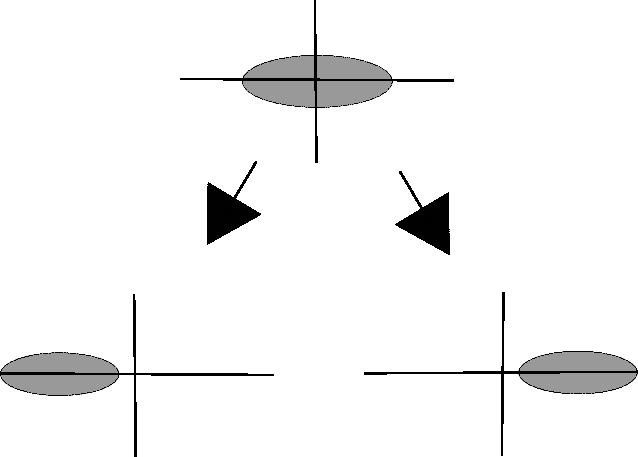
\includegraphics[width=5cm]{DOPO_threshold_phase_portrait} 
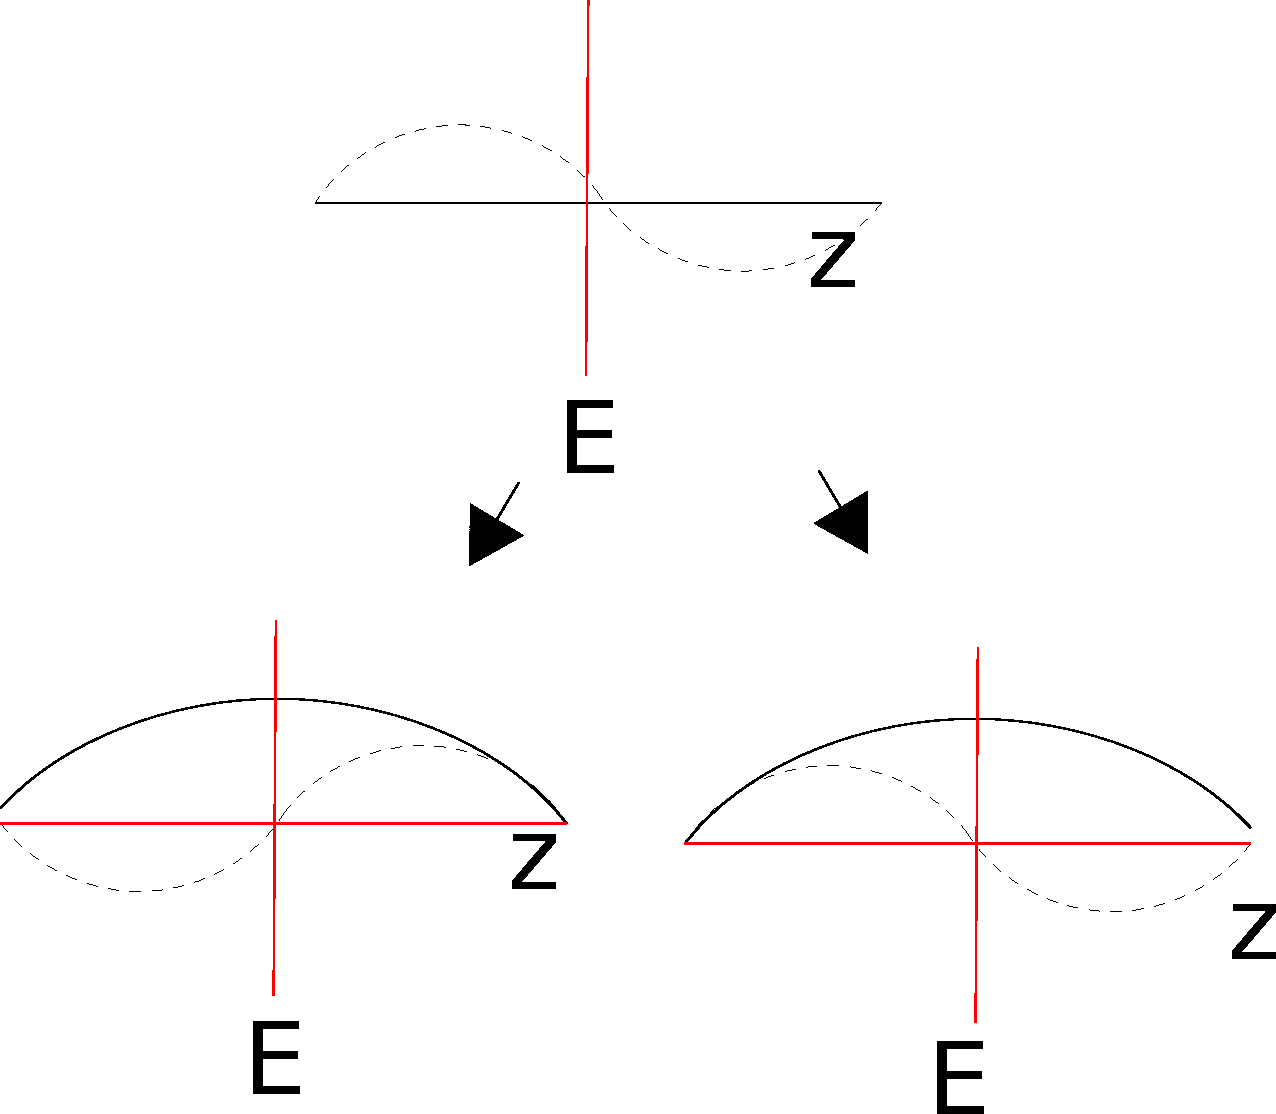
\includegraphics[width=5cm]{DOPO_threshold_fields}
\item But which happens when we cross threshold? If we don't do anything than random fluctuations will select one over the other giving a random result (spontaneous symmetry breaking), if we plot the average over many runs the mean value of the phase will look like a pitchfork, hence this is sometimes called a ``pitchfork'' bifrication
\begin{itemize}
\item But we can also seed a small amount of light with either the $+$ or $-$ phase, the device will amplify that input, using this feedback between multiple modes is the basic operating principle of a coherent Ising machine
\end{itemize}
\end{itemize}

\section{Building a coherent Ising machine}
\begin{itemize}
\item A lot of discussion here taken from Yamamoto et.~al.~npj Quantum Information volume 3, Article number: 49 (2017) \href{https://doi.org/10.1038/s41534-017-0048-9}{https://doi.org/10.1038/s41534-017-0048-9}
\item If our pump beam consists of spatially-separated wave packets, than the OPO will produce multiple wave packets, each with their own phase relationship to the pump beam $\rightarrow$ phase of each effectively acts as a binary (i.e.~Ising) variable above threshold
\item Interaction can be achieved by mixing light from one packet into others, possibly amplifying and modifying the phase (to get anti-ferromagnetic)
\item Threshold will now depend on combination of modes due to feedback, minimum energy configuration will be the first to pass threshold 
\item In principle (fully quantum version):
\begin{itemize}
\item Everything I describe above can be done with delay lines and other optical components
\item If done this way, a coherent Ising machine is a fully quantum model of computing, with no intermediate measurements and full entanglement possible between packets
\item Similar to quantum annealing, except for the fact that more has been proven for quantum annealing (there is an annealing version of the Grover problem with an analogous speedup, I don't think the same exists for coherent Ising\footnote{There is theoretical evidence for quantum correlations and entanglement, see \href{https://arxiv.org/abs/1506.00135}{https://arxiv.org/abs/1506.00135}})
\item This has been done on a small scale ( $4$ variables in Yamamoto et.~al.)
\end{itemize}
\item Diagram of what this looks like (taken from Yamamoto et.~al.)

\begin{centering}
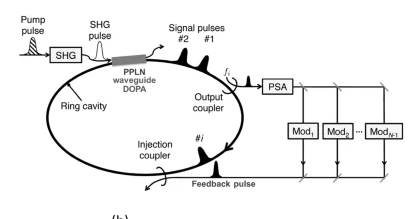
\includegraphics[width=10cm]{delay_CIM_from_Yamamoto}
\par
\end{centering}
\item In practice (classical version):
\begin{itemize}
\item Engineering a large number of interactions using delay lines is not practical from an engineering standpoint
\item But it is possible to measure and create feedback which approximates what delay lines would have given
\item This allows coherence locally, but not entanglement between the packets, still potentially very powerful , but not quantum computing in the way we usually imagine it
\begin{itemize}
\item In particular, lack of coherence between wave packets rules out any kind of Grover type speedup, wavepackets are effectively being used as anlog components within a larger classical computer
\item Having individual quantum components does not make a device a quantum computer, transistors rely on quantum effects to operate but we wouldn't call a laptop or smartphone a quantum computer
\end{itemize}
\item These can be large, and can perform pretty well in practice
\end{itemize}
\item Diagram of what this looks like (taken from Yamamoto et.~al.)

\begin{centering}
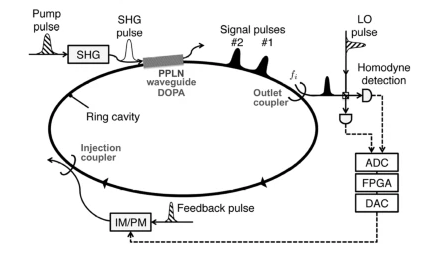
\includegraphics[width=10cm]{classical_CIM_from_Yamamoto}
\par
\end{centering}
\end{itemize}

\section{How to measure out the state of each variable: Homodyne detection}
\begin{itemize}
\item Phase is only defined relative to the local oscillator, therefore to measure out the Ising variables we must use a process known as Homodyne detection (discussed in section 7.3 in G+K)
\item Assume we have a strong light signal at the frequency $\omega_s=\frac{\omega_p}{2}$ produced as part of our laser and in phase with the pump beam (one of the two possible options) if we didn't have this, we could make it with another OPO, it would be squeezed in that case, but this wouldn't affect the basic argument
\item  Now consider that we send these two pulses into a $50:50$ beam splitter, if we use $\hat{a}$ for the light we want to measure and $\hat{b}$ for the reference, we see that the difference in intensity on each arm of the beamsplitter is\footnote{The factor of $i$ which appears in the last expression initially appears alarming, since this is a physical quantity and therefore its expectation should be a real number, however, the quantity within the brackets is \textbf{anti-}Hermitian and therefore will have purely imaginary expectation values, leading to an overall real number}
\begin{align}
I_c-I_d\propto \average{\hat{n}_c-\hat{n}_d}=\average{\hat{c}^\dagger\hat{c}-\hat{d}^\dagger\hat{d}}=\\
\frac{1}{2}\average{(\hat{a}^\dagger-i\hat{b}^\dagger)(\hat{a}+i\hat{b})-(\hat{b}^\dagger-i\hat{a}^\dagger)(\hat{b}+i\hat{a})}=i\average{\hat{a}^\dagger\hat{b}-\hat{a}\hat{b}^\dagger}
\end{align}
\begin{centering}
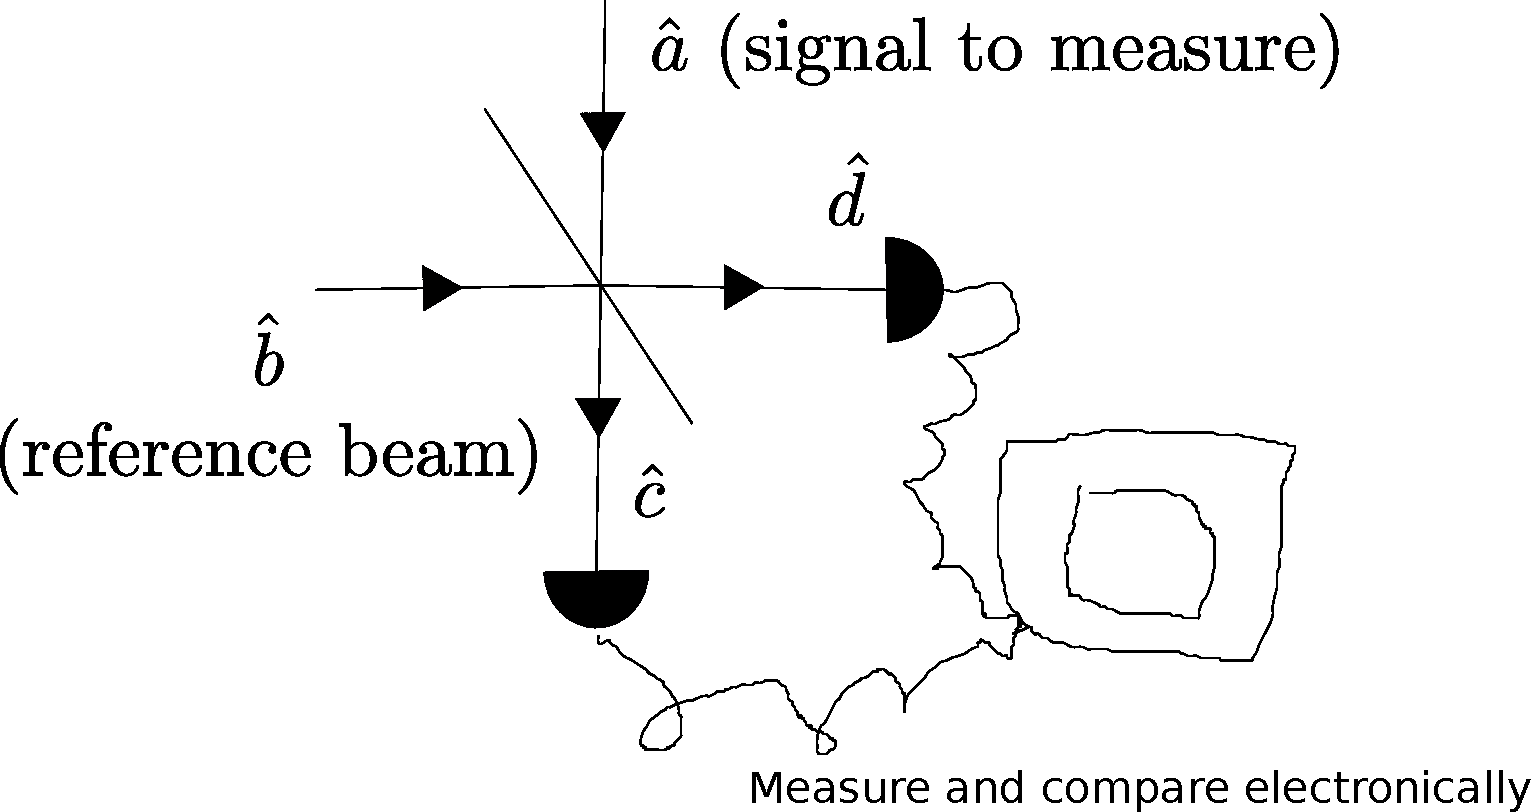
\includegraphics[width=10cm]{homodyne}
\par
\end{centering}
\item If the field associated with $\hat{b}$ is a coherent state described by $\ket{\beta\exp(i \omega_s t)}=\ket{|\beta|\exp(-i \omega_s t+i(\theta-\frac{\pi}{2}))}$, then this expression reduces to something proportional to $\average{\hat{a}^\dagger\exp(i \omega_s t-i \theta)+\hat{a}\exp(-i \omega_s t+i \theta)}$
\item We now observe that $\average{\hat{a}}$ is also time dependent $\average{\hat{a}}=\average{\hat{a}_0}\exp(i \omega_s t)$, plugging this in gives $\average{\hat{a}_0^\dagger\exp(-i \theta)+\hat{a}_0\exp(i \theta)}$, which is exactly a measure of the expectation of the quadrature operator along a direction defined by $\theta$, we can therefore distinguish the states of the Ising variables based on which detector sees more intense light
\item Note that G+K focuses on using this method to measure squeezing by measuring fluctuations in the intensity difference, but can also directly measure the quadrature
\end{itemize}


\end{document}